%------------------------------------------------------------------------------
% beamer_template.tex
%------------------------------------------------------------------------------
%
% Template Author:   Jonathan Duncan
%           Walla Walla University
%           Winter Quarter, 2014
%
%-------------------------------------------------------------
%
% Document Author:  Caleb Bibb
%           Lake City Junior Academy
%           2018-2019
%
%------------------------------------------------------------------

% Document class for presentations or handout
%\documentclass[handout]{beamer}
\documentclass{beamer}

% theme to use -- you can change if you like!
\usetheme{Darmstadt}

% packages to use 
\usepackage{hyperref}
\usepackage{tikz}
\usetikzlibrary{arrows.meta,arrows}
\usepackage{pgfplots}
\pgfplotsset{compat=newest}

% set dynamic uncovering (doesn't work well for images)
\setbeamercovered{dynamic}
%\setbeamercovered{invisible}

% title page
\title{Section 2.7a: Graphing Linear Inequalities}
\author{Caleb Bibb}
\institute{``I can graph inequalities on a number line.''}
%\date{2018}


% set up outline to begin at each section
% \AtBeginSection[]{\frame{\frametitle{Outline}\scriptsize\tableofcontents[current]}}


% now for the actual document
\begin{document}

  % I don't like the navigation symbols, so I turn them off
  \beamertemplatenavigationsymbolsempty

  % the title page
  \frame{\titlepage}
  
  % an outline of the talk
%  \frame{\frametitle{Outline}\scriptsize\tableofcontents}

  % a section (can have multiple ones)
  \section{Graphing with Inequalities}
    \frame{
      \frametitle{Graphing Inequalities on the number line}
    \begin{example}
    $<$ and $>$ use hollow points and are the same as $($ and $)$
        \begin{center}
        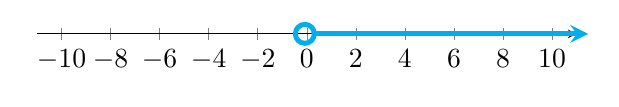
\begin{tikzpicture}
            \begin{axis}[
                xtick={-10,-8,...,10},
                axis x line=bottom,
                xmin=-11,
                xmax=11,
                hide y axis,
                ymin=0,
                ymax=1,
            ]
            \end{axis}
            \draw[o-stealth, thick, cyan, line width=1.8pt]{(3.25,0) -- (7,0)};
        \end{tikzpicture}
		$$(0,\infty) \text{ or } 0<x $$
        \end{center}
    \end{example}
    \begin{example}
    $\leq$ and $\geq$ use solid points and are the same as $[$ and $]$
        \begin{center}
        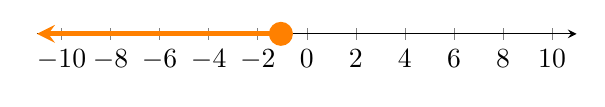
\begin{tikzpicture}
            \begin{axis}[
                xtick={-10,-8,...,10},
                axis x line=bottom, % only show the bottom x axis
                xmin=-11,
                xmax=11,
                hide y axis,
                ymin=-1,
                ymax=1,
            ]
            \end{axis}
			\draw[*-stealth, thick, orange, line width=1.8pt]{(3.25,0) -- (0,0)};
        \end{tikzpicture}
		$$(-\infty, -1] \text{ or } x\leq -1$$
        \end{center}
    \end{example}
    }
    \frame{
    \frametitle{We Do 1:}
    \begin{example}
    Graph $x>2$ \\
    \begin{center}
        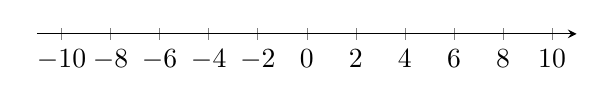
\begin{tikzpicture}
            \begin{axis}[
                xtick={-10,-8,...,10},
                axis x line=bottom, % only show the bottom x axis
                xmin=-11,
                xmax=11,
                hide y axis,
                ymin=0,
                ymax=1,
            ]
            \end{axis}
        \end{tikzpicture}
    \end{center}
    \end{example}
	\begin{example}
    Graph $[2,\infty)$ \\
    \begin{center}
        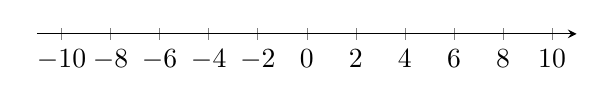
\begin{tikzpicture}
            \begin{axis}[
                xtick={-10,-8,...,10},
                axis x line=bottom, % only show the bottom x axis
                xmin=-11,
                xmax=11,
                hide y axis,
                ymin=0,
                ymax=1,
            ]
            \end{axis}
        \end{tikzpicture}
    \end{center}
    \end{example}
    }
\frame{
    \frametitle{You Do 1:}
    \begin{alertblock}{You Do 1a}
    Graph $x<4$ \\
    \begin{center}
        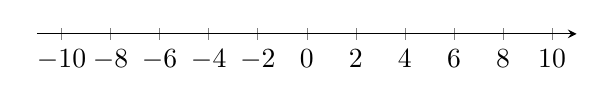
\begin{tikzpicture}
            \begin{axis}[
                xtick={-10,-8,...,10},
                axis x line=bottom, % only show the bottom x axis
                xmin=-11,
                xmax=11,
                hide y axis,
                ymin=0,
                ymax=1,
            ]
            \end{axis}
        \end{tikzpicture}
    \end{center}
    \end{alertblock}
	\begin{alertblock}{You Do 1b}
    Graph $[-2,\infty)$ \\
    \begin{center}
        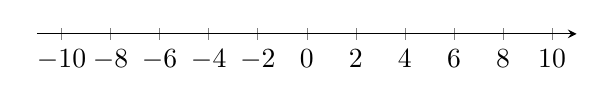
\begin{tikzpicture}
            \begin{axis}[
                xtick={-10,-8,...,10},
                axis x line=bottom, % only show the bottom x axis
                xmin=-11,
                xmax=11,
                hide y axis,
                ymin=0,
                ymax=1,
            ]
            \end{axis}
        \end{tikzpicture}
    \end{center}
    \end{alertblock}
}
\frame{
    \frametitle{You Do 2:}
    \begin{alertblock}{You Do 2a}
    Graph $x\geq3$ \\
    \begin{center}
        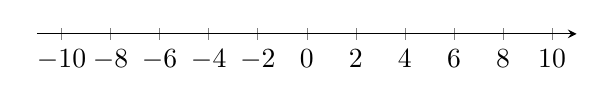
\begin{tikzpicture}
            \begin{axis}[
                xtick={-10,-8,...,10},
                axis x line=bottom, % only show the bottom x axis
                xmin=-11,
                xmax=11,
                hide y axis,
                ymin=0,
                ymax=1,
            ]
            \end{axis}
        \end{tikzpicture}
    \end{center}
    \end{alertblock}
	\begin{alertblock}{You Do 2b}
    Graph $(-\infty,\frac{3}{4})$ \\
    \begin{center}
        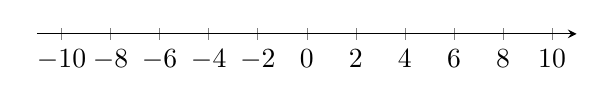
\begin{tikzpicture}
            \begin{axis}[
                xtick={-10,-8,...,10},
                axis x line=bottom, % only show the bottom x axis
                xmin=-11,
                xmax=11,
                hide y axis,
                ymin=0,
                ymax=1,
            ]
            \end{axis}
        \end{tikzpicture}
    \end{center}
    \end{alertblock}
}
\end{document}